\chapter{Výsledky}
Zkoumali jsme molekuly $\mathrm{BeH/BeH^-}$ a $\mathrm{OH/OH^-}$, protože se jedná o 
molekuly, které mají vázaný jak základní stav, tak anion, a zároveň se jedná o 
dostatečně malé systémy, aby bylo možné provádět výpočty přesnými metodami.

Ke kvantově chemickým výpočtům jsme používali program MOLPRO.\cite{MOLPRO-WIREs}\cite{MOLPRO}. 
Pro určitý soubor mezijaderných vzdáleností\footnote{cca 35 hodnot} jsme napočítali 
energii základního stavu molekuly pro fixovaná jádra, u základního stavu, tak u 
aniontu. Ze znalosti těchto křivek jsme poté zjišťovali parametry molekul, které je 
možné nalézt experimentálně, což jsou disociační energie aniontu i neutrální molekuly a 
elektronové afinity vázané i úplně disociované\footnote{Ta odpovídá odpovídá 
elektronové afinitě některého z prvků v molekule.} molekuly. Protože ale experimentální 
data nejsou určená minimem potenciální energie molekuly, ale základní vibrační 
hladinou, bylo třeba napočítat energetické hladiny získaného potenciálu. K tomu jsme 
použili \? metodu výpočtu na na mříži \? . Vzhledem k počtu geometrií, pro které jsme 
prováděli kvantově-chemické výpočty, který byl nedostatečný pro další numerické výpočty
\footnote{a extrémní výpočetní náročnosti při případném výpočtu v dostatečném počtu 
geometrií}, jsme získané hodnoty proložili kubickým splinem, ze kterého jsme pak 
interpolovali hodnotu potenciálu v několika stovkách bodů. Poté jsme numericky získali 
energetické hladiny v daném potenciálové křivce pro částici o (redukované) hmotnosti $
\mu = m_1m_2/(m_1+m_2)$, kde $m_1,m_2$ jsou hmotnosti jednotlivých jader. Získané 
vlastní stavy pak odpovídají vibračním stavům dané molekuly.

\begin{figure}
\centering
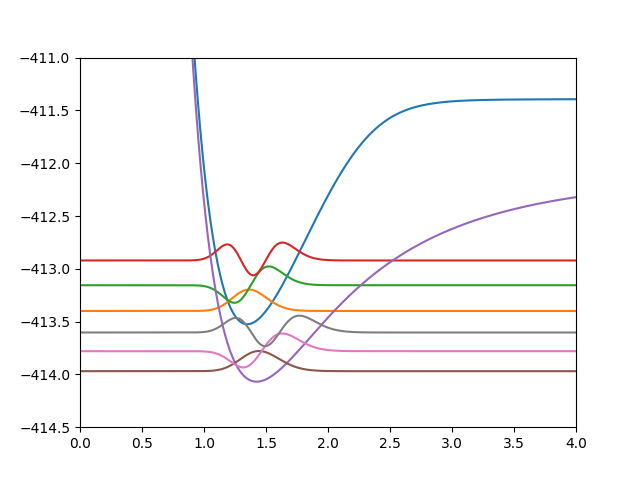
\includegraphics[width=0.8\textwidth]{../img/VibrStavy1.png}
\caption{Nejnižší vibrační hladiny molekul $\mathrm{BeH/BeH^-}$}
\label{Vibr1}
\end{figure}


\centering
\label{TODO}
\begin{tabular}{rrrrr}
\toprule
Method & $E_a(BeH)[" eV"]$ & $E_a(H)[" eV"]$ & $D_a(BeH)[" eV"]$ & $D_a(BeH^-)[" eV"]$ \\ \midrule
    Experimental:  & $0.70\pm0.1$ & $0.754195$        & $2.18\pm0.02$ & $2.07$ \\ \midrule
FCI  /aug-cc-pVDZ & 0.542 & 0.679 & 1.895 & 1.759\\
RCCSD(T)  /aug-cc-pVDZ & 0.534 & 0.679 & 1.888 & 1.744\\
CI 5,1,1,0 /aug-cc-pVDZ & 0.536 & -0.325 & 1.892 & 2.753\\
CI 6,2,2,0 /aug-cc-pVDZ & 0.542 & 0.678 & 1.893 & 1.756\\
FCI  /aug-cc-pCVDZ & 0.546 & 0.679 & 1.901 & 1.769\\
RCCSD(T)  /aug-cc-pCVDZ & 0.538 & 0.679 & 1.894 & 1.753\\
CI 5,1,1,0 /aug-cc-pCVDZ & 0.540 & 0.603 & 1.898 & 1.835\\
CI 6,2,2,0 /aug-cc-pCVDZ & 0.528 & 0.670 & 1.899 & 1.756\\
FCI  /cc-pVTZ & 0.326 & -0.091 & 1.990 & 2.407\\
RCCSD(T)  /cc-pVTZ & 0.320 & -0.091 & 1.983 & 2.394\\
CI 6,2,2,0 /cc-pVTZ & 0.325 & -0.091 & 1.988 & 2.404\\
FCI  /aug-cc-pVTZ & 0.570 & 0.734 & 2.010 & 1.847\\
RCCSD(T)  /aug-cc-pVTZ & 0.562 & 0.734 & 2.003 & 1.832\\
CI 6,2,2,0 /aug-cc-pVTZ & 0.569 & 0.732 & 2.006 & 1.844\\
RCCSD(T)  /aug-cc-pVQZ & 0.566 & 0.746 & 2.034 & 1.854\\
CI 5,1,1,0 /aug-cc-pVQZ & 0.565 & 0.744 & 2.038 & 1.858\\
CI 6,2,2,0 /aug-cc-pVQZ & 0.572 & 0.746 & 2.039 & 1.865\\
CI 9,3,3,1 /aug-cc-pVQZ & 0.573 & 0.746 & 2.039 & 1.867\\
CI 5,1,1,0 /aug-cc-pV5Z & 0.567 & 0.750 & 2.044 & 1.862\\
CI 6,2,2,0 /aug-cc-pV5Z & 0.575 & 0.752 & 2.046 & 1.869\\
\bottomrule
\end{tabular}

    
\begin{tabular}{rrrrr}
\toprule
Method & $v_0 [\mathrm{eV}]$ & $v_1 [\mathrm{eV}]$ & $v_2 [\mathrm{eV}]$ & $v_3[\mathrm{eV}]$ \\ \midrule
    FCI  /aug-cc-pVDZ & 0.1240 & 0.3648 & 0.5953 & 0.8152\\
RCCSD(T)  /aug-cc-pVDZ & 0.1244 & 0.3661 & 0.5975 & 0.8186\\
CI 5,1,1,0 /aug-cc-pVDZ & 0.1240 & 0.3649 & 0.5954 & 0.8153\\
CI 6,2,2,0 /aug-cc-pVDZ & 0.1240 & 0.3648 & 0.5953 & 0.8152\\
FCI  /aug-cc-pCVDZ & 0.1245 & 0.3658 & 0.5966 & 0.8168\\
RCCSD(T)  /aug-cc-pCVDZ & 0.1249 & 0.3670 & 0.5988 & 0.8201\\
CI 5,1,1,0 /aug-cc-pCVDZ & 0.1245 & 0.3658 & 0.5967 & 0.8169\\
CI 6,2,2,0 /aug-cc-pCVDZ & 0.1245 & 0.3658 & 0.5966 & 0.8168\\
FCI  /cc-pVTZ & 0.1254 & 0.3688 & 0.6021 & 0.8252\\
RCCSD(T)  /cc-pVTZ & 0.1257 & 0.3698 & 0.6039 & 0.8281\\
CI 6,2,2,0 /cc-pVTZ & 0.1254 & 0.3688 & 0.6021 & 0.8252\\
FCI  /aug-cc-pVTZ & 0.1252 & 0.3682 & 0.6010 & 0.8234\\
RCCSD(T)  /aug-cc-pVTZ & 0.1255 & 0.3692 & 0.6028 & 0.8263\\
CI 6,2,2,0 /aug-cc-pVTZ & 0.1254 & 0.3691 & 0.6032 & 0.8275\\
RCCSD(T)  /aug-cc-pVQZ & 0.1261 & 0.3713 & 0.6065 & 0.8314\\
CI 5,1,1,0 /aug-cc-pVQZ & 0.1258 & 0.3704 & 0.6047 & 0.8287\\
CI 6,2,2,0 /aug-cc-pVQZ & 0.1258 & 0.3704 & 0.6047 & 0.8286\\
CI 9,3,3,1 /aug-cc-pVQZ & 0.1258 & 0.3704 & 0.6047 & 0.8286\\
CI 5,1,1,0 /aug-cc-pV5Z & 0.1259 & 0.3707 & 0.6052 & 0.8293\\
CI 6,2,2,0 /aug-cc-pV5Z & 0.1259 & 0.3707 & 0.6052 & 0.8293\\
\bottomrule
\end{tabular}
    
\label{TODO}
\begin{tabular}{rrrrr}
\toprule
Method & $E_a(OH)[" eV"]$ & $E_a(O)[" eV"]$ & $D_a(OH)[" eV"]$ & $D_a(OH^-)[" eV"]$ \\ \midrule
Experimental:  & $1.82767$ & $1.461$ &        $4.3914$ & $5.120435$ \\ \midrule
CI 4,1,1,0 /aug-cc-pVDZ & 1.345 & -1.637 & 4.054 & 7.035\\
CI 4,2,2,0 /aug-cc-pVDZ & 1.559 & 1.084 & 4.090 & 4.565\\
CI 6,2,2,0 /aug-cc-pVDZ & 1.609 & 1.182 & 4.104 & 4.531\\
CI 8,2,2,0 /aug-cc-pVDZ & 1.614 & 1.188 & 4.101 & 4.527\\
CI 4,1,1,0 /aug-cc-pVTZ & 1.376 & -1.517 & 4.234 & 7.127\\
CI 4,2,2,0 /aug-cc-pVTZ & 1.629 & 1.158 & 4.269 & 4.739\\
CI 6,2,2,0 /aug-cc-pVTZ & 1.687 & 1.303 & 4.306 & 4.690\\
CI 8,2,2,0 /aug-cc-pVTZ & 1.693 & 1.308 & 4.296 & 4.681\\
CI 4,1,1,0 /aug-cc-pVQZ & 1.413 & -1.480 & 4.292 & 7.185\\
CI 4,2,2,0 /aug-cc-pVQZ & 1.674 & 1.218 & 4.332 & 4.789\\
CI 6,2,2,0 /aug-cc-pVQZ & 1.733 & 1.362 & 4.369 & 4.740\\
CI 8,2,2,0 /aug-cc-pVQZ & 1.740 & 1.368 & 4.359 & 4.730\\
\bottomrule
\end{tabular}
    
\begin{table}[]
\centering
\caption{OH vibration states}
\label{TODO}
\begin{tabular}{rrrrr}
\toprule
Method & $v_0 [" eV"]$ & $v_1 [" eV"]$ & $v_2 [" eV"]$ & $v_3[" eV"]$ \\ \midrule
CI 4,1,1,0 /aug-cc-pVDZ & 0.225 & 0.657 & 1.065 & 1.451\\
CI 4,2,2,0 /aug-cc-pVDZ & 0.224 & 0.656 & 1.063 & 1.448\\
CI 6,2,2,0 /aug-cc-pVDZ & 0.224 & 0.656 & 1.064 & 1.450\\
CI 8,2,2,0 /aug-cc-pVDZ & 0.224 & 0.656 & 1.063 & 1.449\\
CI 4,1,1,0 /aug-cc-pVTZ & 0.227 & 0.665 & 1.081 & 1.474\\
CI 4,2,2,0 /aug-cc-pVTZ & 0.227 & 0.664 & 1.078 & 1.469\\
CI 6,2,2,0 /aug-cc-pVTZ & 0.227 & 0.664 & 1.079 & 1.473\\
CI 8,2,2,0 /aug-cc-pVTZ & 0.227 & 0.664 & 1.078 & 1.471\\
CI 4,1,1,0 /aug-cc-pVQZ & 0.228 & 0.668 & 1.085 & 1.481\\
CI 4,2,2,0 /aug-cc-pVQZ & 0.227 & 0.665 & 1.080 & 1.474\\
CI 6,2,2,0 /aug-cc-pVQZ & 0.227 & 0.667 & 1.084 & 1.479\\
CI 8,2,2,0 /aug-cc-pVQZ & 0.227 & 0.666 & 1.083 & 1.477\\
\bottomrule
\end{tabular}
\end{table}
    
\begin{tabular}{rrrrr}
\toprule
Method & $v_0 [\mathrm{eV}]$ & $v_1 [\mathrm{eV}]$ & $v_2 [\mathrm{eV}]$ & $v_3[\mathrm{eV}]$ \\ \midrule
CI 4,1,1,0 /aug-cc-pVDZ & 0.228 & 0.662 & 1.069 & 1.449\\
CI 4,2,2,0 /aug-cc-pVDZ & 0.221 & 0.647 & 1.047 & 1.426\\
CI 6,2,2,0 /aug-cc-pVDZ & 0.224 & 0.655 & 1.059 & 1.440\\
CI 8,2,2,0 /aug-cc-pVDZ & 0.224 & 0.653 & 1.057 & 1.437\\
CI 4,1,1,0 /aug-cc-pVTZ & 0.212 & 0.637 & 1.047 & 1.448\\
CI 4,2,2,0 /aug-cc-pVTZ & 0.221 & 0.649 & 1.054 & 1.439\\
CI 6,2,2,0 /aug-cc-pVTZ & 0.225 & 0.661 & 1.072 & 1.460\\
CI 8,2,2,0 /aug-cc-pVTZ & 0.225 & 0.660 & 1.070 & 1.457\\
CI 4,1,1,0 /aug-cc-pVQZ & 0.212 & 0.637 & 1.052 & 1.455\\
CI 4,2,2,0 /aug-cc-pVQZ & 0.224 & 0.657 & 1.066 & 1.450\\
CI 6,2,2,0 /aug-cc-pVQZ & 0.225 & 0.663 & 1.077 & 1.467\\
CI 8,2,2,0 /aug-cc-pVQZ & 0.225 & 0.662 & 1.075 & 1.463\\
\bottomrule
\end{tabular}
    